\documentclass{article}
\usepackage[utf8]{inputenc}
\usepackage{multicol}
\usepackage{listings}
\usepackage{verbatim}
\usepackage{color}
\usepackage{geometry}
\usepackage{float}
\usepackage{amsmath}
\usepackage{hyperref}
\setlength{\belowcaptionskip}{-10pt}
\setlength{\abovecaptionskip}{-30pt}
\floatstyle{boxed} 
\restylefloat{figure}
\usepackage{graphicx}
\definecolor{codegreen}{rgb}{0,0.6,0}
\definecolor{codegray}{rgb}{0.5,0.5,0.5}
\definecolor{codepurple}{rgb}{0.58,0,0.82}
\definecolor{backcolour}{rgb}{0.95,0.95,0.92}

\lstdefinestyle{mystyle}{
	backgroundcolor=\color{backcolour},   
	commentstyle=\color{codegreen},
	keywordstyle=\color{blue},
	numberstyle=\tiny\color{codegray},
	stringstyle=\color{codepurple},
	basicstyle=\footnotesize,
	breakatwhitespace=false,         
	breaklines=true,                 
	captionpos=b,                    
	keepspaces=true,                 
	numbers=left,                    
	numbersep=5pt,                  
	showspaces=false,                
	showstringspaces=false,
	showtabs=false,                  
	tabsize=2
}

\lstset{style=mystyle}
\title{Data Mining\\
		Home work 06\\Association rules, 2x2 tables, interestingness}
\author{Aqeel Labash\\ \textbf{Lecturer:} Jaak Vilo}
\date{17 March 2016}

\geometry{
	a4paper,
	total={170mm,257mm},
	left=10mm,
	top=5mm,
}
\begin{document}
	\maketitle
	\section*{First Question}
\setlength{\columnsep}{20pt}
\begin{multicols}{2}

	For this task I implemented it on python and here is the code for it : 
	\begin{lstlisting}[language=python]
# coding: utf-8

# In[96]:

import itertools
import sys


# In[97]:

main =[]
main.append(sorted(['B','C', 'A' ,'F', 'H']))
main.append(sorted(['F', 'E', 'C', 'H']))
main.append(sorted(['E' ,'D', 'B']))
main.append(sorted(['A', 'C' ,'H', 'F']))
main.append(sorted(['E', 'F' ,'A']))
main.append(sorted(['D', 'H' ,'B']))
main.append(sorted(['E', 'C' ,'F', 'B', 'D']))
main.append(sorted(['A', 'H' ,'C', 'E']))
main.append(sorted(['G', 'A', 'E']))
main.append(sorted(['B', 'H', 'E']))


# In[98]:

class Core:
def __init__(self,name=None,occurence=0):
self.name = name
self.occurence =occurence
self.sons={}
def AddItem(self,items):
if len(items)<=0:
return
if items[0] in self.sons.keys():
self.sons[items[0]].occurence+=1
self.sons[items[0]].AddItem(items[1:])
else:
self.sons[items[0]] = Core(name=items[0],occurence=1)
self.sons[items[0]].AddItem(items[1:])
def printeverything(self,level=0):
#print 
thespace = '----'*level
print(thespace+str(self.name)+':'+str(self.occurence))
for itm in self.sons.keys():
self.sons[itm].printeverything(level=level+1)
#sys.stdout.write('\n')
#def printeverything2(self,level=0):
#    print '\t' * level + repr(self.value)
#    for child in self.children:
#        child.other_name(level+1)


# In[99]:

nullobject = Core()
for item in main:
nullobject.AddItem(item)


# In[100]:

nullobject.printeverything()
	\end{lstlisting}
And the result tree was like this :
None:0\\
----A:5\\
--------C:2\\
------------E:1\\
----------------H:1\\
------------F:1\\
----------------H:1\\
--------B:1\\
------------C:1\\
----------------F:1\\
--------------------H:1\\
--------E:2\\
------------G:1\\
------------F:1\\
----C:1\\
--------E:1\\
------------F:1\\
----------------H:1\\
----B:4\\
--------C:1\\
------------D:1\\
----------------E:1\\
--------------------F:1\\
--------E:1\\
------------H:1\\
--------D:2\\
------------H:1\\
------------E:1\\
\end{multicols}
The following picture is what (me \& faiz) draw on the board:
\begin{figure}[H]
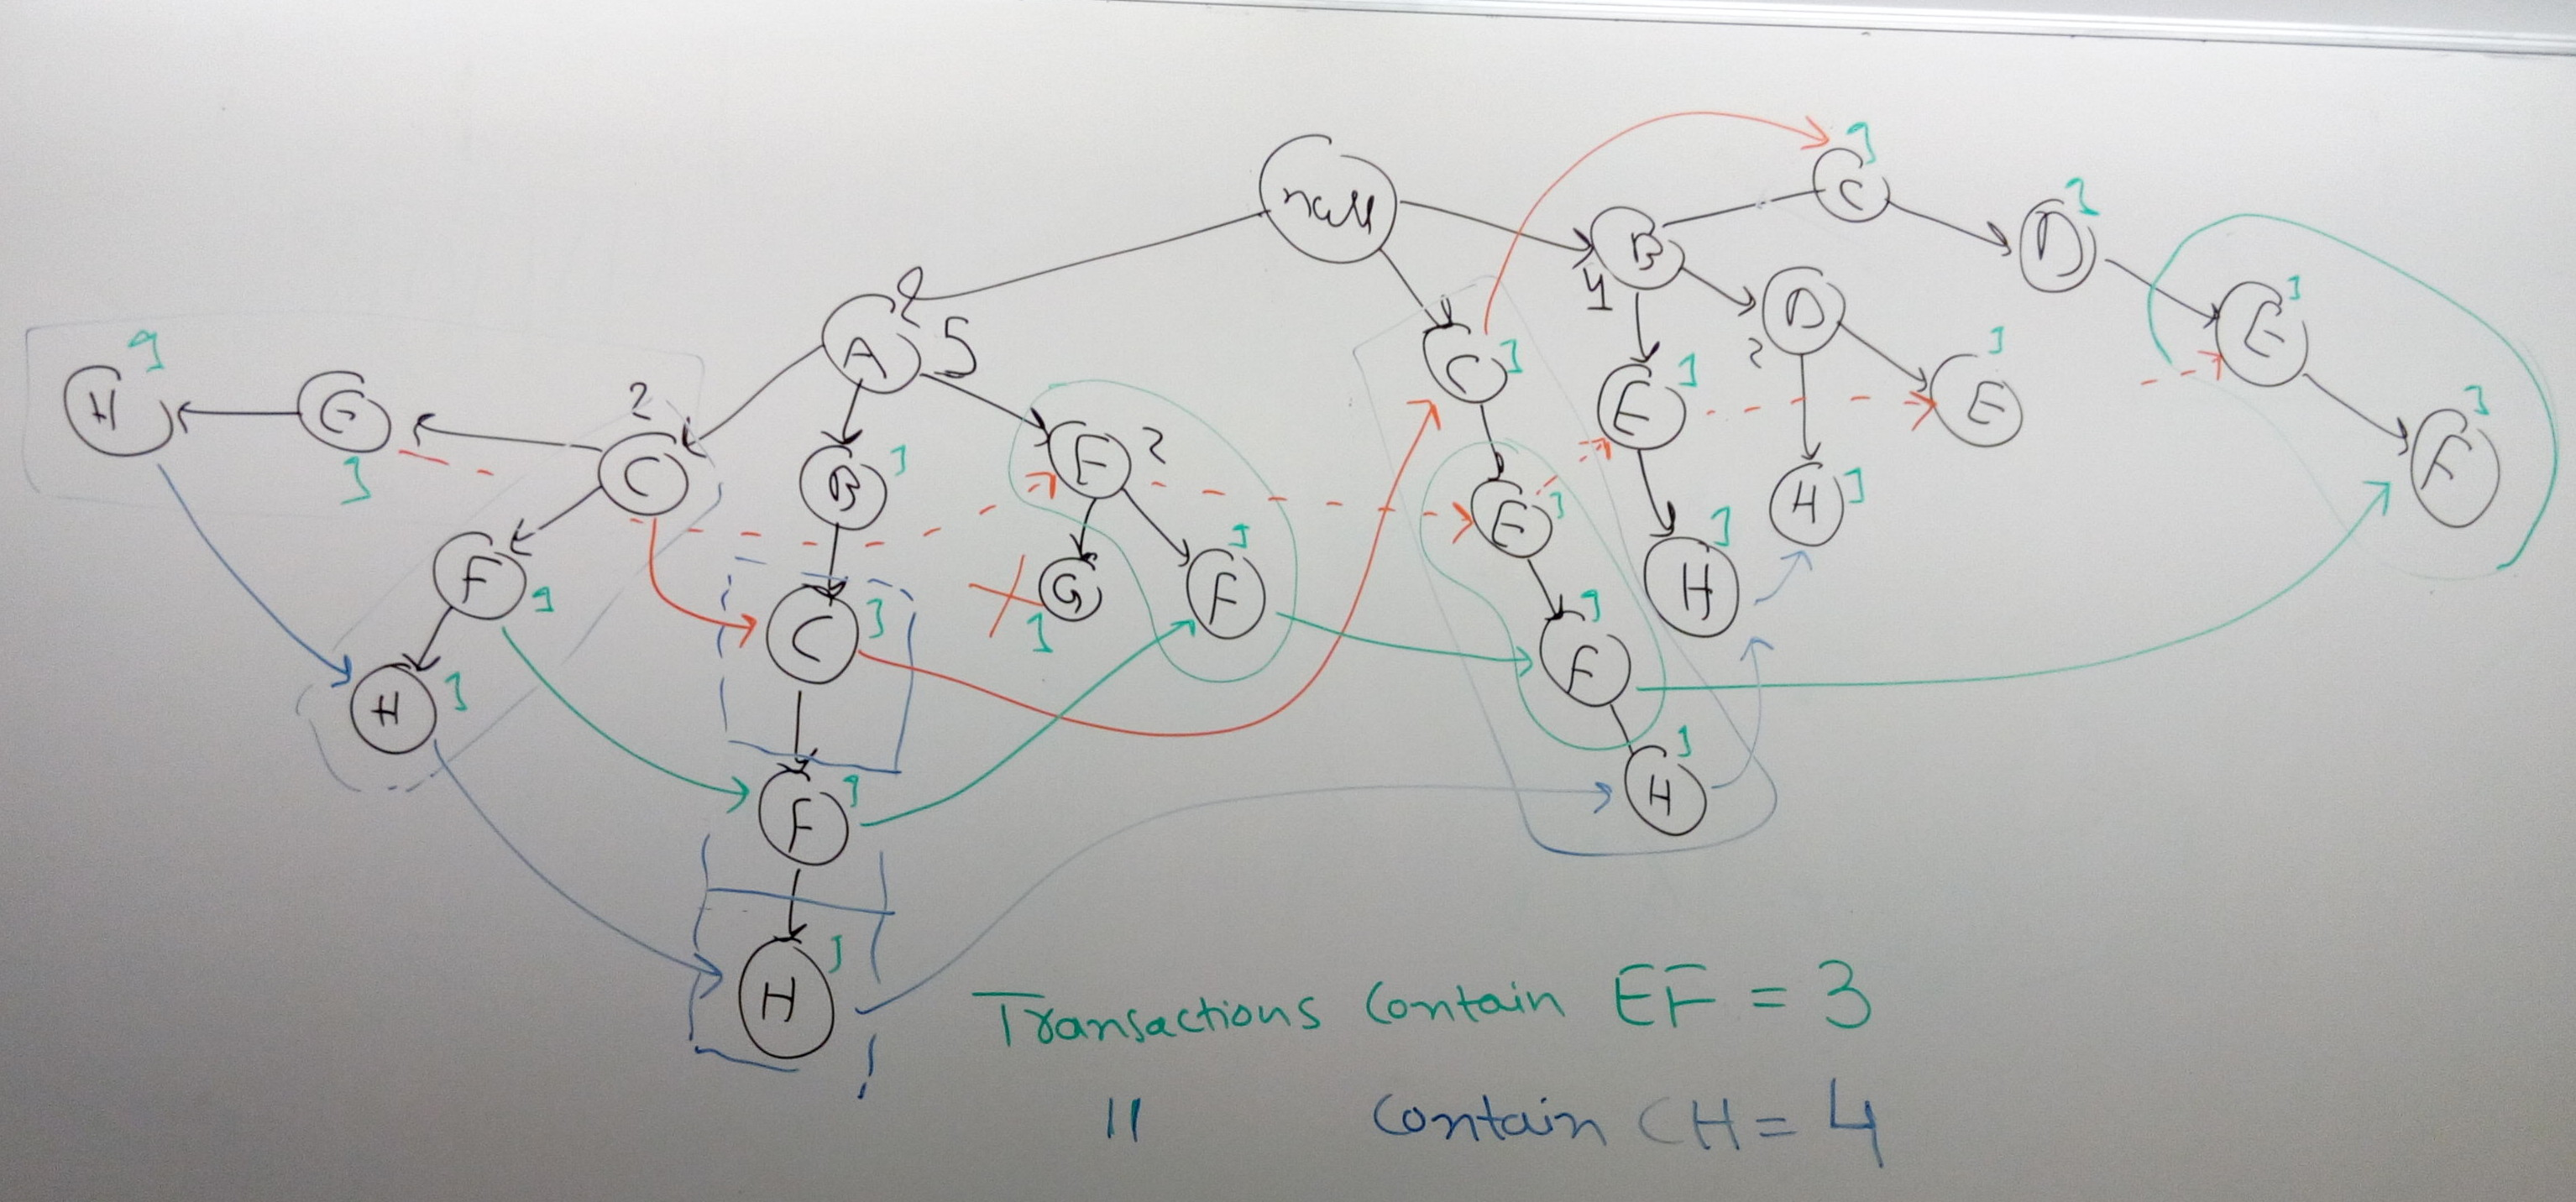
\includegraphics[scale=0.15]{board.jpg}
\caption{Image show the elements graph}
\end{figure}
How we build it:
\begin{enumerate}
	\item Put null node at the start.
	\item start adding transactions one by one
	\item when the an element of the transaction already exist I just increase it's occurrence number and pass the rest of the transaction to it and so on.
\end{enumerate}
The number of transaction that contain EF = 3.\\
The number of transaction that contain CH = 4.
	\section*{Second Question}
For this I question I used python and here is the code :
\begin{lstlisting}[language=python]

# coding: utf-8

# In[462]:

import numpy as np
import itertools
from math import sqrt
rnd.seed(4)


# In[463]:

class AllNeeded:
def __init__(self,value):
self.f11=value[0]
self.f10=value[1]
self.f01=value[2]
self.f00=value[3]
self.f1plus= self.f11+self.f10
self.f0plus= self.f01+self.f00
self.fplus1= self.f11+self.f01
self.fplus0=self.f10+self.f00
#self.oddsratio = float(self.f11*self.f00)/self.isZero( float(self.f10*self.f01))
self.all_confidence = min(float(self.f11)/float(self.f1plus),float(self.f11)/float(self.fplus1))
self.kappa = float(10000*self.f11+10000*self.f00-self.f1plus*self.fplus1-
self.f0plus*self.fplus0) /float(100000000-self.f1plus*self.fplus1-self.f0plus*self.fplus0)
self.interest = float(10000*self.f11)/float(self.f1plus*self.fplus1)
self.cosine= float(self.f11)/float(sqrt(self.f1plus*self.fplus1))
self.Jaccard = float(self.f11)/float(self.f1plus+self.fplus1-self.f11)

def isZero(self,value):
return 1 if value==0 else value
def __str__(self):
return 'f11:{},f10:{},f01:{},f00:{},f1+:{},f0+:{},f+1:{},f+0:{}'.format(self.f11,self.f10,self.f01,
self.f00,self.f1plus,self.f0plus,
self.fplus1,self.fplus0)




# To generate 4 numbers sum to 10000 I used 
# #Create the array
#     #result =np.random.dirichlet(np.ones(4),size=1)
# #multilply with 10,000 (so The sum is 10,000)
#     #result = result *10000
# #Convert the array to type int
#     result =np.array( result,dtype=int)
# # add 2 to one of the array elements to recover the loset precesion
#     result[0,np.random.randint(4)]+=2
#     

# In[464]:

lst = []
total =np.array(np.random.dirichlet(np.ones(4),size=10000)*10000,dtype=int)
for result in total:
result[np.random.randint(4,size=1)]+=(10000-np.sum(result))
lst.append(AllNeeded(result))


# In[478]:

allconf = sorted(lst,key=lambda x:x.all_confidence,reverse=True)[:10]
print '=========All Confidence=============='
for element in allconf:
print element,',all_confidence :',element.all_confidence

print '========= kappa =============='
allconf = sorted(lst,key=lambda x:x.kappa,reverse=True)[:10]
for element in allconf:
print element,',kappa :',element.kappa
print '========= interest =============='
allconf = sorted(lst,key=lambda x:x.interest,reverse=True)[:10]
for element in allconf:
print element,',interest :',element.interest
print '========= cosine =============='
allconf = sorted(lst,key=lambda x:x.cosine,reverse=True)[:10]
for element in allconf:
print element,',cosine :',element.cosine
print '========= Jaccard =============='
allconf = sorted(lst,key=lambda x:x.Jaccard,reverse=True)[:10]
for element in allconf:
print element,',Jaccard :',element.Jaccard
\end{lstlisting}
and the output as following : \\
=========All Confidence==============
f11:8802,f10:31,f01:21,f00:1146,f1+:8833,f0+:1167,f+1:8823,f+0:1177 ,all\_confidence : 0.996490433601\\
f11:7915,f10:11,f01:49,f00:2025,f1+:7926,f0+:2074,f+1:7964,f+0:2036 ,all\_confidence : 0.993847312908\\
f11:8185,f10:9,f01:72,f00:1734,f1+:8194,f0+:1806,f+1:8257,f+0:1743 ,all\_confidence : 0.991280125954\\
f11:4120,f10:45,f01:38,f00:5797,f1+:4165,f0+:5835,f+1:4158,f+0:5842 ,all\_confidence : 0.989195678271\\
f11:7964,f10:20,f01:123,f00:1893,f1+:7984,f0+:2016,f+1:8087,f+0:1913 ,all\_confidence : 0.984790404353\\
f11:3193,f10:52,f01:24,f00:6731,f1+:3245,f0+:6755,f+1:3217,f+0:6783 ,all\_confidence : 0.983975346687\\
f11:6363,f10:115,f01:39,f00:3483,f1+:6478,f0+:3522,f+1:6402,f+0:3598 ,all\_confidence : 0.982247607286\\
f11:8778,f10:169,f01:23,f00:1030,f1+:8947,f0+:1053,f+1:8801,f+0:1199 ,all\_confidence : 0.981110986923\\
f11:8308,f10:197,f01:6,f00:1489,f1+:8505,f0+:1495,f+1:8314,f+0:1686 ,all\_confidence : 0.976837154615\\
f11:6308,f10:162,f01:17,f00:3513,f1+:6470,f0+:3530,f+1:6325,f+0:3675 ,all\_confidence : 0.974961360124\\
========= kappa ==============\\
f11:4120,f10:45,f01:38,f00:5797,f1+:4165,f0+:5835,f+1:4158,f+0:5842 ,kappa : 0.982919652812\\
f11:3193,f10:52,f01:24,f00:6731,f1+:3245,f0+:6755,f+1:3217,f+0:6783 ,kappa : 0.982625263279\\
f11:7915,f10:11,f01:49,f00:2025,f1+:7926,f0+:2074,f+1:7964,f+0:2036 ,kappa : 0.981625906394\\
f11:8802,f10:31,f01:21,f00:1146,f1+:8833,f0+:1167,f+1:8823,f+0:1177 ,kappa : 0.974870585934\\
f11:8185,f10:9,f01:72,f00:1734,f1+:8194,f0+:1806,f+1:8257,f+0:1743 ,kappa : 0.972254842763\\
f11:5187,f10:7,f01:159,f00:4647,f1+:5194,f0+:4806,f+1:5346,f+0:4654 ,kappa : 0.966710619345\\
f11:6363,f10:115,f01:39,f00:3483,f1+:6478,f0+:3522,f+1:6402,f+0:3598 ,kappa : 0.966416380014\\
f11:3435,f10:105,f01:54,f00:6406,f1+:3540,f0+:6460,f+1:3489,f+0:6511 ,kappa : 0.965122308824\\
f11:2850,f10:129,f01:27,f00:6994,f1+:2979,f0+:7021,f+1:2877,f+0:7123 ,kappa : 0.962335974982\\
f11:2266,f10:93,f01:44,f00:7597,f1+:2359,f0+:7641,f+1:2310,f+0:7690 ,kappa : 0.961722669847\\
========= interest ==============\\
f11:165,f10:312,f01:154,f00:9369,f1+:477,f0+:9523,f+1:319,f+0:9681 ,interest : 10.8436347864\\
f11:478,f10:185,f01:201,f00:9136,f1+:663,f0+:9337,f+1:679,f+0:9321 ,interest : 10.6180457909\\
f11:304,f10:118,f01:444,f00:9134,f1+:422,f0+:9578,f+1:748,f+0:9252 ,interest : 9.63073725828\\
f11:328,f10:610,f01:58,f00:9004,f1+:938,f0+:9062,f+1:386,f+0:9614 ,interest : 9.05907177657\\
f11:137,f10:939,f01:16,f00:8908,f1+:1076,f0+:8924,f+1:153,f+0:9847 ,interest : 8.32179216172\\
f11:415,f10:440,f01:176,f00:8969,f1+:855,f0+:9145,f+1:591,f+0:9409 ,interest : 8.21286153907\\
f11:932,f10:14,f01:279,f00:8775,f1+:946,f0+:9054,f+1:1211,f+0:8789 ,interest : 8.13543225158\\
f11:216,f10:945,f01:13,f00:8826,f1+:1161,f0+:8839,f+1:229,f+0:9771 ,interest : 8.12430181781\\
f11:984,f10:73,f01:293,f00:8650,f1+:1057,f0+:8943,f+1:1277,f+0:8723 ,interest : 7.29002829331\\
f11:716,f10:402,f01:185,f00:8697,f1+:1118,f0+:8882,f+1:901,f+0:9099 ,interest : 7.10798377474\\
========= cosine ==============\\
f11:8802,f10:31,f01:21,f00:1146,f1+:8833,f0+:1167,f+1:8823,f+0:1177 ,cosine : 0.997054985476\\
f11:7915,f10:11,f01:49,f00:2025,f1+:7926,f0+:2074,f+1:7964,f+0:2036 ,cosine : 0.996226888987\\
f11:8185,f10:9,f01:72,f00:1734,f1+:8194,f0+:1806,f+1:8257,f+0:1743 ,cosine : 0.995083583875\\
f11:7964,f10:20,f01:123,f00:1893,f1+:7984,f0+:2016,f+1:8087,f+0:1913 ,cosine : 0.991122340845\\
f11:4120,f10:45,f01:38,f00:5797,f1+:4165,f0+:5835,f+1:4158,f+0:5842 ,cosine : 0.990027984416\\
f11:8778,f10:169,f01:23,f00:1030,f1+:8947,f0+:1053,f+1:8801,f+0:1199 ,cosine : 0.98921535114\\
f11:3193,f10:52,f01:24,f00:6731,f1+:3245,f0+:6755,f+1:3217,f+0:6783 ,cosine : 0.988248212585\\
f11:6363,f10:115,f01:39,f00:3483,f1+:6478,f0+:3522,f+1:6402,f+0:3598 ,cosine : 0.988060679228\\
f11:8308,f10:197,f01:6,f00:1489,f1+:8505,f0+:1495,f+1:8314,f+0:1686 ,cosine : 0.98799402648\\
f11:6308,f10:162,f01:17,f00:3513,f1+:6470,f0+:3530,f+1:6325,f+0:3675 ,cosine : 0.986073481348\\
========= Jaccard ==============\\
f11:8802,f10:31,f01:21,f00:1146,f1+:8833,f0+:1167,f+1:8823,f+0:1177 ,Jaccard : 0.994126948272\\
f11:7915,f10:11,f01:49,f00:2025,f1+:7926,f0+:2074,f+1:7964,f+0:2036 ,Jaccard : 0.992476489028\\
f11:8185,f10:9,f01:72,f00:1734,f1+:8194,f0+:1806,f+1:8257,f+0:1743 ,Jaccard : 0.990200822647\\
f11:7964,f10:20,f01:123,f00:1893,f1+:7984,f0+:2016,f+1:8087,f+0:1913 ,Jaccard : 0.982360922659\\
f11:4120,f10:45,f01:38,f00:5797,f1+:4165,f0+:5835,f+1:4158,f+0:5842 ,Jaccard : 0.980252200809\\
f11:8778,f10:169,f01:23,f00:1030,f1+:8947,f0+:1053,f+1:8801,f+0:1199 ,Jaccard : 0.978595317726\\
f11:3193,f10:52,f01:24,f00:6731,f1+:3245,f0+:6755,f+1:3217,f+0:6783 ,Jaccard : 0.976751300092\\
f11:6363,f10:115,f01:39,f00:3483,f1+:6478,f0+:3522,f+1:6402,f+0:3598 ,Jaccard : 0.976369495166\\
f11:8308,f10:197,f01:6,f00:1489,f1+:8505,f0+:1495,f+1:8314,f+0:1686 ,Jaccard : 0.976148513688\\
f11:6308,f10:162,f01:17,f00:3513,f1+:6470,f0+:3530,f+1:6325,f+0:3675 ,Jaccard : 0.972406351164\\
More explanation about those method and how I generated them in the ipython file attached with home work or you can find it on \href{https://github.com/aqeel13932/DM/tree/master/HW06}{github,Q2.ipython}
	\section*{Third Question}
	For this question I used the previous code and added the following code :
	\begin{lstlisting}[language = Python]
	x = range(1000)
	labels = []
	plotHandles = []
	y1 = [AllNeeded((i,250,250,250)) for i in x]
	#for i in range(1, num_plots + 1):
	t, = plt.plot(x, [y.all_confidence for y in y1]) #need the ',' per ** below
	plotHandles.append(t)
	labels.append('All Confidence')
	t, = plt.plot(x, [y.kappa for y in y1]) #need the ',' per ** below
	plotHandles.append(t)
	labels.append('kappa')
	t, = plt.plot(x, [y.interest for y in y1]) #need the ',' per ** below
	plotHandles.append(t)
	labels.append('interest')
	t, = plt.plot(x, [y.cosine+0.1 for y in y1]) #need the ',' per ** below
	plotHandles.append(t)
	labels.append('cosine + 0.1')
	t, = plt.plot(x, [y.Jaccard for y in y1]) #need the ',' per ** below
	plotHandles.append(t)
	labels.append('Jaccard')
	plt.legend(plotHandles, labels, 'upper left',loc=1)
	plt.show()
	
	labels = []
	plotHandles = []
	y1 = [AllNeeded((250,i,250,250)) for i in x]
	#for i in range(1, num_plots + 1):
	t, = plt.plot(x, [y.all_confidence for y in y1]) #need the ',' per ** below
	plotHandles.append(t)
	labels.append('All Confidence')
	t, = plt.plot(x, [y.kappa for y in y1]) #need the ',' per ** below
	plotHandles.append(t)
	labels.append('kappa')
	t, = plt.plot(x, [y.interest for y in y1]) #need the ',' per ** below
	plotHandles.append(t)
	labels.append('interest')
	t, = plt.plot(x, [y.cosine for y in y1]) #need the ',' per ** below
	plotHandles.append(t)
	labels.append('cosine')
	t, = plt.plot(x, [y.Jaccard for y in y1]) #need the ',' per ** below
	plotHandles.append(t)
	labels.append('Jaccard')
	plt.legend(plotHandles, labels, 'upper left',loc=1)
	plt.show()
	
	labels = []
	plotHandles = []
	y1 = [AllNeeded((250,250,i,250)) for i in x]
	#for i in range(1, num_plots + 1):
	t, = plt.plot(x, [y.all_confidence for y in y1]) #need the ',' per ** below
	plotHandles.append(t)
	labels.append('All Confidence')
	t, = plt.plot(x, [y.kappa for y in y1]) #need the ',' per ** below
	plotHandles.append(t)
	labels.append('kappa')
	t, = plt.plot(x, [y.interest for y in y1]) #need the ',' per ** below
	plotHandles.append(t)
	labels.append('interest')
	t, = plt.plot(x, [y.cosine for y in y1]) #need the ',' per ** below
	plotHandles.append(t)
	labels.append('cosine')
	t, = plt.plot(x, [y.Jaccard for y in y1]) #need the ',' per ** below
	plotHandles.append(t)
	labels.append('Jaccard')
	plt.legend(plotHandles, labels, 'upper left',loc=1)
	plt.show()
	
	labels = []
	plotHandles = []
	y1 = [AllNeeded((250,250,250,i)) for i in x]
	#for i in range(1, num_plots + 1):
	t, = plt.plot(x, [y.all_confidence for y in y1]) #need the ',' per ** below
	plotHandles.append(t)
	labels.append('All Confidence')
	t, = plt.plot(x, [y.kappa for y in y1]) #need the ',' per ** below
	plotHandles.append(t)
	labels.append('kappa')
	t, = plt.plot(x, [y.interest for y in y1]) #need the ',' per ** below
	plotHandles.append(t)
	labels.append('interest')
	t, = plt.plot(x, [y.cosine+0.1 for y in y1]) #need the ',' per ** below
	plotHandles.append(t)
	labels.append('cosine+0.1')
	t, = plt.plot(x, [y.Jaccard for y in y1]) #need the ',' per ** below
	plotHandles.append(t)
	labels.append('Jaccard')
	plt.legend(plotHandles, labels, 'upper left',loc=1)
	plt.show()
	\end{lstlisting}
	The previous code generate 4 plots. each plot represent how the change in the value in one of(f11,f10,f01,f00) would affect the measurements.
	\begin{figure}[H]
		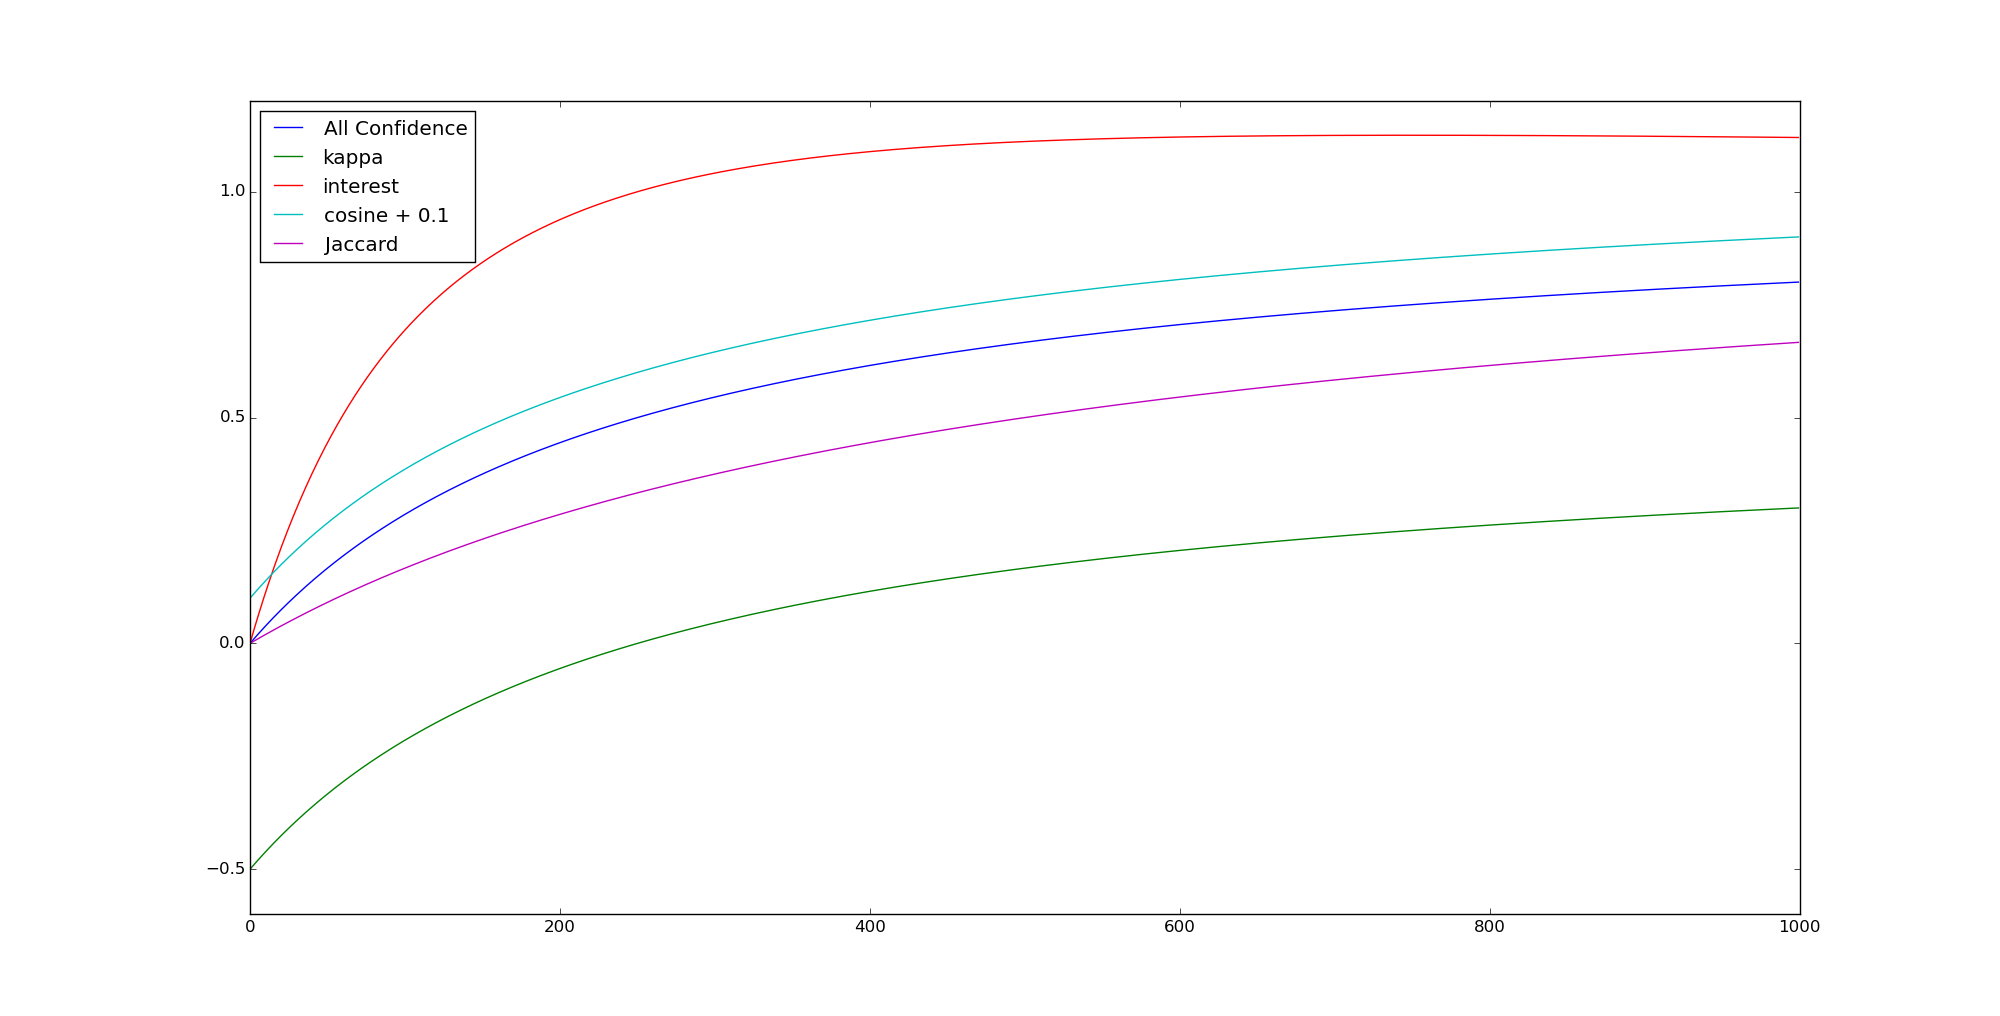
\includegraphics[scale=0.35]{f11.png}
		\caption{The measurements while changing f11}
	\end{figure}
	In this figure I believe all the the measurements have a logarithmic growth when we change f11.
	\begin{figure}[H]
		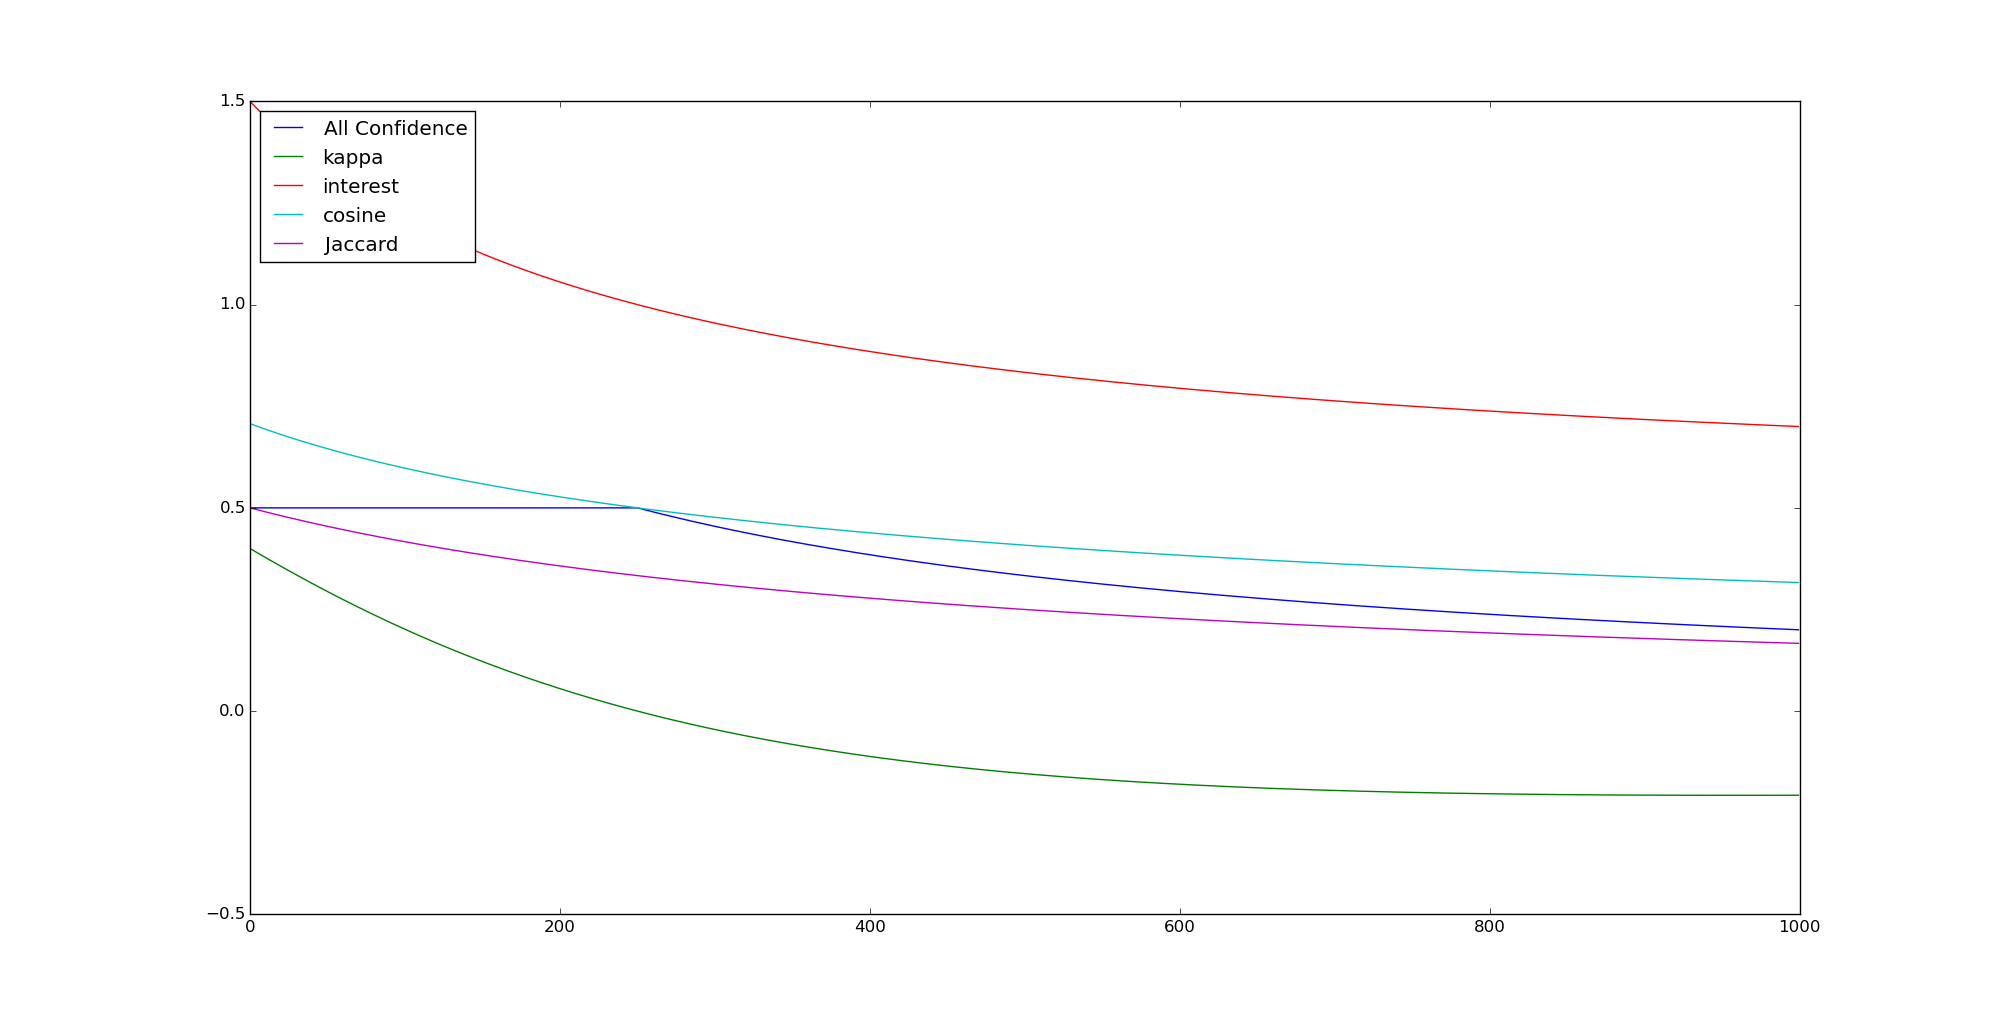
\includegraphics[scale=0.35]{f10.png}
		\caption{The measurements while changing f10}
	\end{figure}
In figure 3 I think we have -log growth for all the measurements 
	\begin{figure}[H]
		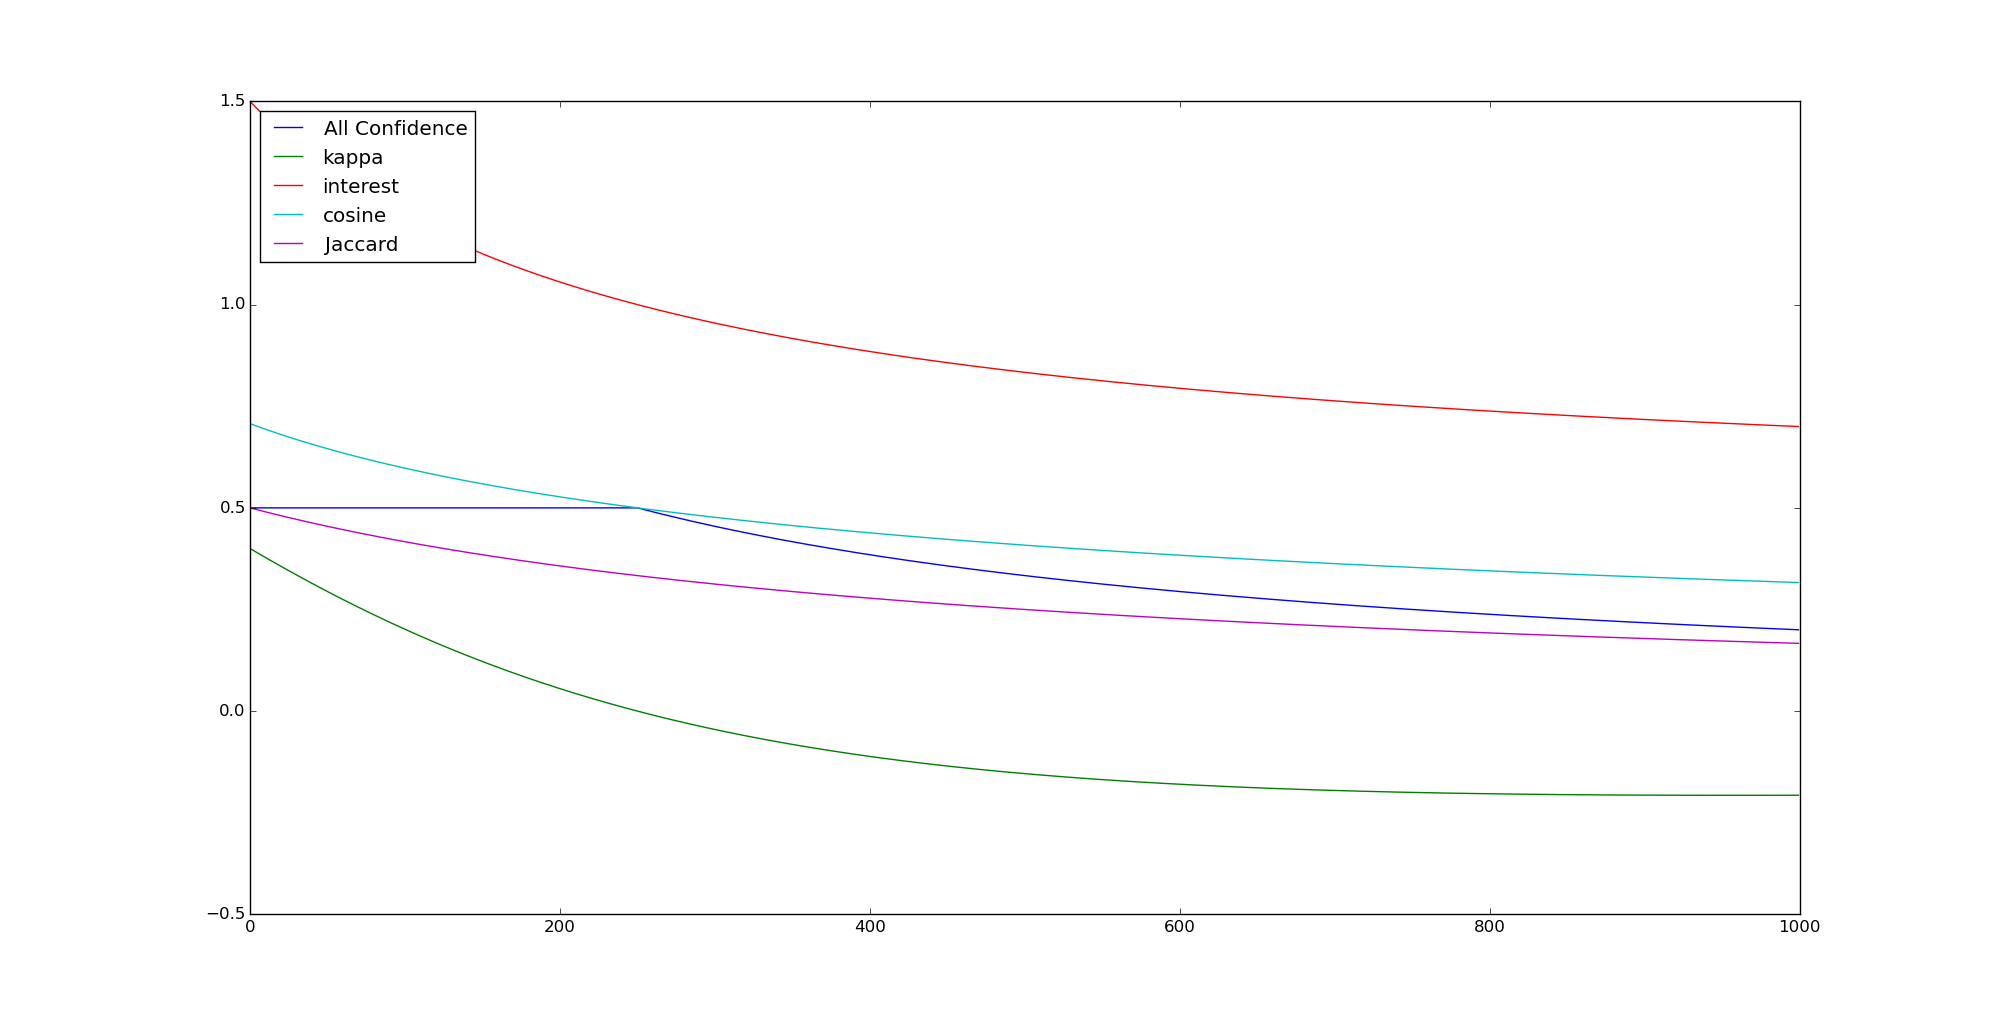
\includegraphics[scale=0.35]{f01.png}
		\caption{The measurements while changing f01}
	\end{figure}
	In figure 4 I would say they have same behavior as figure 3 except All confidence 
	\begin{figure}[H]
		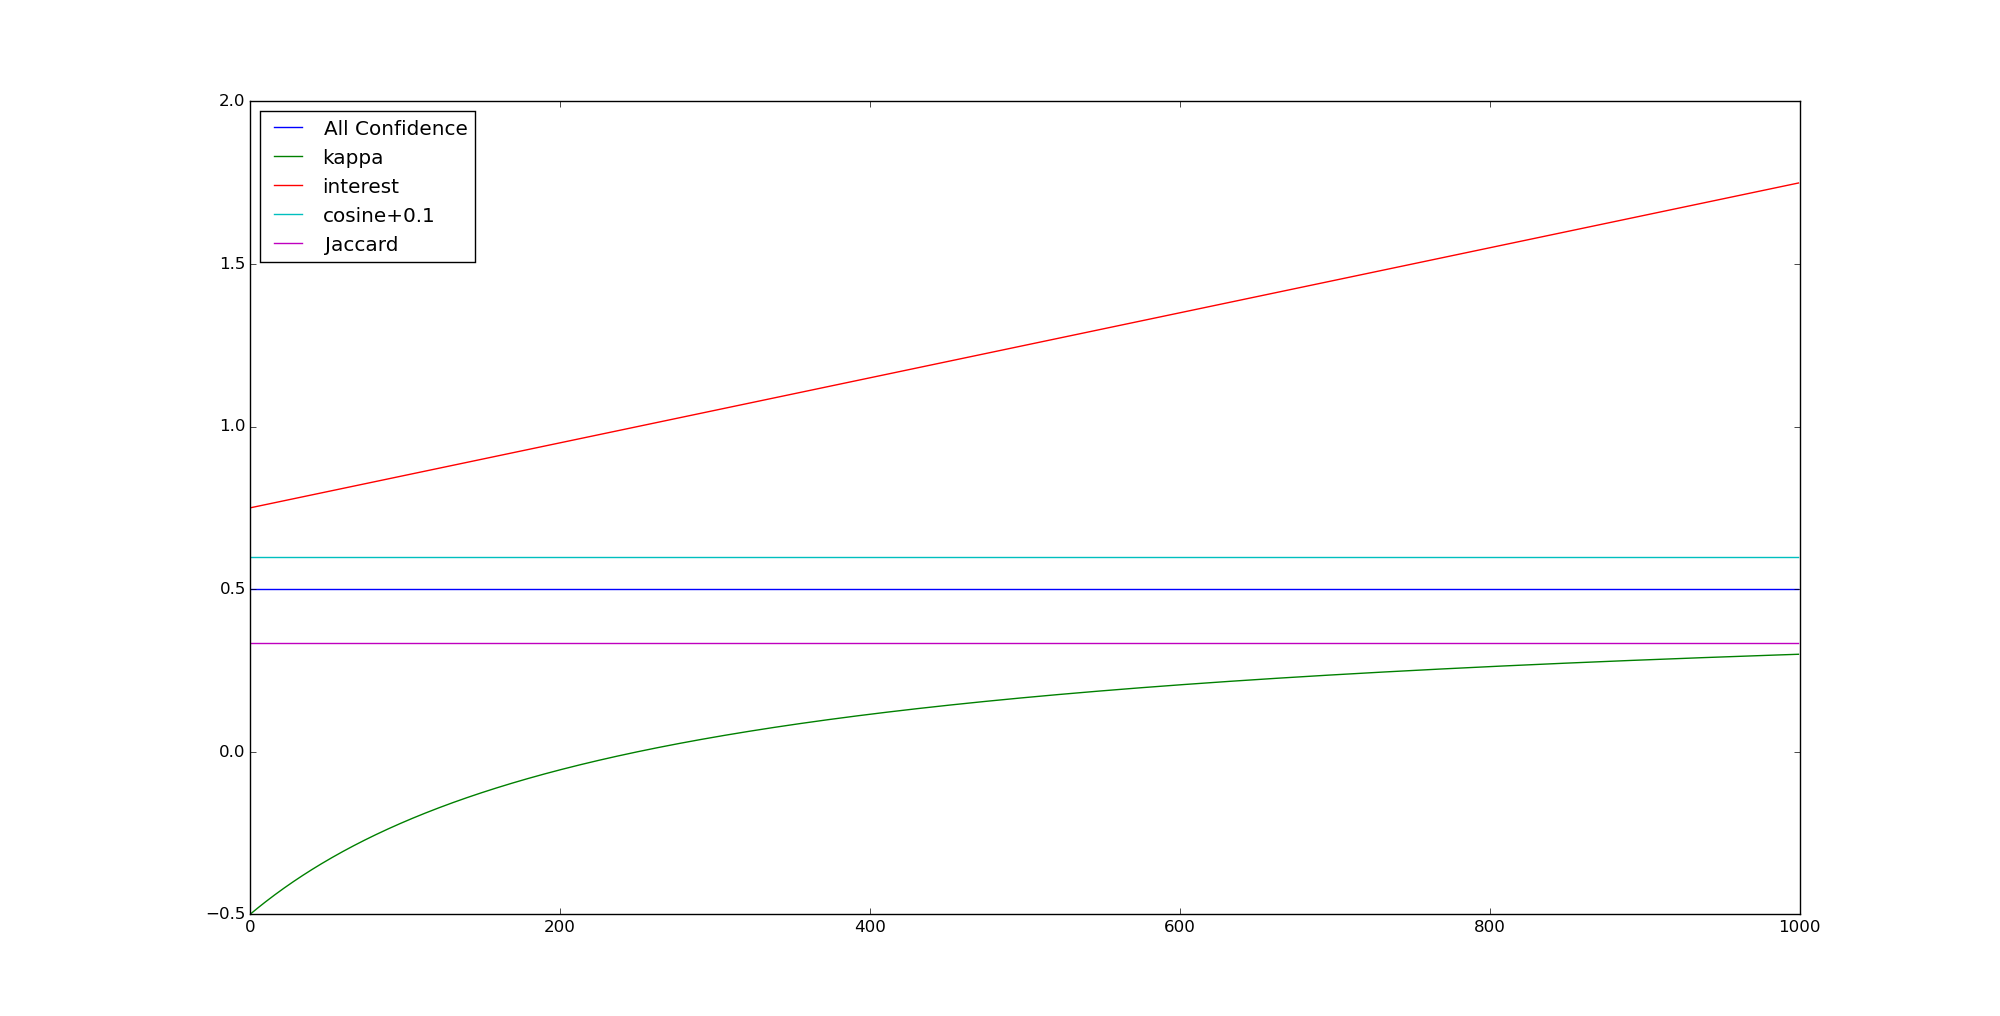
\includegraphics[scale=0.35]{f00.png}
		\caption{The measurements while changing f00}
	\end{figure}
In figure 5 I think we can see that interest is linear with f00 , kappa is logarithmic, the rest doesn't get affected at all. 
	\section*{Fourth Question}
	\section*{Fifth Question}
	\section*{Sixth Question}
					
\end{document}